\projectstart{c2}{C2}{Convertidor A/D}

\section{Objectius}

En aquesta pràctica s'introdueix el Conversor Analògic a Digital (ADC)
de la placa, s'explica breument el funcionament i l'us, i es fa servir
per mesurar la posició del potenciòmetre, la temperatura i el voltatge
de referència. Aquest últim, al seu torn, es fa servir per calibrar la segona mesura.

\section{Desenvolupament}


\subsection{Descripció del convertidor ADC}

Es comença exposant les especificacions i característiques dels convertidors
A/D de la placa. Concretament farem servir l'ADC~1. S'explica l'estructura
interna de l'ADC, les 19 entrades de les que disposa, internes i externes,
com funcionen les seqüències regulars i com funcionen les injectades, a quins
registres s'emmagatzemen els resultats en cada cas, i el rellotge de l'ADC.

\subsection{Configuració de l'ADC 1}

Ara s'aprofundeix en l'us de l'ADC des del software; quins passos calen
al nostre codi per a habilitar i configurar correctament el perifèric.

En concret, es demana com a estudi previ triar un valor per a configurar
el \emph{prescaler} del rellotge de l'ADC, per tal de derivar-lo amb la freqüència
adequada per al perifèric:

%previ
Segons el datasheet dels STM32F407xx (pàg.~118) i per a \(V_{DDA} = \SI{3.3}{\volt}\), PCLK2 hauria d'estar
entre \SI{0.6}{\mega\hertz} i \SI{36}{\mega\hertz}, i el seu valor típic és \SI{30}{\mega\hertz}.

Com que no tenim cap preferència concreta, triarem el valor que més s'apropi al típic (respectant els límits).
Aquest valor és \mintinline{c}{0b01} (PCLK2 es divideix per 4) el qual dona una freqüència de rellotge 
\(f_c = \SI{21}{\mega\hertz}\).
%/previ

Continuant, cal determinar el temps de lectura per a cada canal. S'explica
la necessitat d'ajustar-lo correctament. Com que de moment només volem
mesurar un sol canal (el potenciòmetre), es presenta un circuit simplificat
del potenciòmetre connectat amb l'ADC. A partir d'aquí es demana com
a estudi previ, calcular el temps de lectura mínim per tal que no hi hagi
soroll en les mesures del convertidor:

%previ
Em primer lloc, com diu l'enunciat considerarem negligible la capacitat paràsita, per tant \(C_{parasitic} = 0\).
Notem que els díodes només s'activen quan \(0 - V_x > V_t \Leftrightarrow V_x < -V_t\) i quan \(V_x - V_{dd} > V_t \Leftrightarrow V_x > V_{dd} + V_t\),
i com que la tensió al pin $V_x$ sempre estarà dins \([0, V_{dd}]\) això no es donarà mai. Negligim també l'efecte de les pèrdues de corrent (\(I_L = 0\)).

El circuit resultant és:

\begin{center} \begin{circuitikz} \draw
  (0,0) to[V=$V_{AIN}$] (0,2) to[R=$R_{AIN} + R_{ADC}$] (3,2) to[C=$C_{ADC}$] (3,0) node[rground] {}
  (0,0) node[rground] {}
  (3,2) to[short, *-o] (4,2) node[anchor=west] {$V_o$}
; \end{circuitikz} \end{center}

Un RC senzill amb \(\tau = \left(R_{AIN} + R_{ADC}\right) C_{ADC}\).

La diferència entre $V_o$ i $V_{AIN}$ correspon a:
%
\begin{equation*}
  V_R(t) = \left(V_{AIN} - V_o'\right) e^{-t/\tau}
\end{equation*}
%
Busquem la $t$ mínima que compleixi \( \left|V_R(t)\right| < \frac{V_{dd}}{2^{13}} \):
%
\begin{align*}
  \left|V_{AIN} - V_o'\right| e^{-t/\tau} &< \frac{V_{dd}}{2^{13}}
\\
  -t/\tau &< \ln \left( \frac{V_{dd}}{2^{13}\left|V_{AIN} - V_o'\right|} \right)
\\
  t &> \tau \cdot \ln \left( \frac{2^{13}\left|V_{AIN} - V_o'\right|}{V_{dd}} \right)
\end{align*}
%
Fent l'equivalent de Thevenin del circuit del potenciòmetre, \(V_{AIN} = x V_{dd}\) i \(R_{AIN} = \SI{120}{\ohm} +
\SI{10}{\kilo\ohm} \cdot x(1-x)\). Per tant, posant-nos en el pitjor cas, \(R_{AIN} = \SI{370}{\ohm}; R_{ADC} = \SI{6}{\kilo\ohm};
C_{ADC} = \SI{4}{\pico\farad}; \left|V_{AIN} - V_o'\right| = V_{dd} \):
%
\begin{align*}
  t &> \left( \SI{6}{\kilo\ohm} + \SI{370}{\ohm} \right) \cdot \SI{4}{\pico\farad} \cdot \ln (2^{13})
\\
  t_{Smin} &\simeq \SI{230}{\nano\second}
\end{align*}

El mínim nombre de cicles de lectura requerit, a una freqüència de rellotge de \SI{21}{\mega\hertz} com s'ha determinat abans,
és de \(t_S \cdot f_c \simeq 4.83\). El primer valor del registre que hi arriba és \mintinline{c}{0b001} (15 cicles).

El temps total de conversió ve donat per \(f_c^{-1} \left( n_S + n_B \right)\), que amb \(n_S = 15; n_B = 12; f_c = \SI{21}{\mega\hertz}\)
resulta ser \(t_{Tot} \simeq \SI{1.286}{\micro\second}\).
%/previ

Ara que ja tenim determinats aquests valors només queda posar el pin del potenciòmetre
(PB0) en mode entrada analògica per tal que es connecti al canal IN8 de l'ADC; finalment activem l'ADC.

Es demana, com a estudi previ, implementar la funció \fname{initADC} que farà totes
aquestes inicialitzacions:

%previ
\begin{minted}[mathescape]{c}
// Initialize the ADC peripheral and GPIO pins
void initADC(void) {
    // Enable clock on ADC1
    RCC->APB2ENR = RCC_APB2ENR_ADC1EN;

    // Program ADC clock prescaler as $f_c(APB2) / 4 = \SI{21}{\mega\hertz}$
    ADC->CCR = (ADC->CCR & (~ADC_CCR_ADCPRE)) | ADC_CCR_ADCPRE_DIV4;

    // Set PB0 as analog input (IN8) and disconnect pull ups
    GPIOB->MODER = (GPIOB->MODER & (~GPIO_MODER_MODER0)) | (0b11 * GPIO_MODER_MODER0_0);
    GPIOB->PUPDR = (GPIOB->PUPDR & (~GPIO_PUPDR_PUPDR0));
    // Program sample time for IN8
    ADC1->SMPR2 = (ADC1->SMPR2 & (~ADC_SMPR2_SMP8)) | ADC_SMPR2_SMP_AN8(ADC_SAMPLE_15);

    // Power up ADC1
    ADC1->CR2 |= ADC_CR2_ADON;
}
\end{minted}
\vskip -1em
%/previ


\subsection{Lectura d'un canal amb l'ADC 1}

S'explica ara el procediment de lectura, també des del punt de vista de
la programació. S'explica quins registres serveixen per programar el
canal (o la seqüència de canals, encara que en el nostre cas només farem
una única conversió en un únic canal) i quins registres serveixen per
disparar la conversió, comprovar si ha acabat, i llegir-ne el valor.

Ara es demana, com a estudi previ, fer una funció \fname{readIN8} que
configuri el canal IN8 per a la seva lectura, dispari la conversió,
esperi a que estigui acabada i retorni el valor llegit.

\opcional
Per a simplificar el codi, es fa una funció adicional \fname{readChannel}
que llegeix un canal arbitrari de l'ADC~1:

\begin{minted}{c}
// Read a single specified ADC channel
//      channel  : ADC channel to read
int32_t readChannel(int32_t channel) {
    // Program channel to be read
    ADC1->SQR3 = (ADC1->SQR3 & (~ADC_SQR3_SQ1)) | ADC_SQR3_SQ1_N(channel);

    // Start conversion!
    ADC1->CR2 |= ADC_CR2_SWSTART;

    // Wait for conversion to end
    while ((ADC1->SR & ADC_SR_EOC) == 0);

    // Read converted value
    return ADC1->DR & ADC_DR_DATA;
}
\end{minted}
\vskip -1em

\voluntari
Per millorar la qualitat del codi es declara una constant al header
associada al número de canal del potenciòmetre:

\begin{minted}{c}
#define ADC_CHANNEL_POT (ADC_CHANNEL_IN8)
\end{minted}
\vskip -1em

S'ha seguit la nomenclatura de ChibiOS, que ja defineix \mintinline{c}|ADC_CHANNEL_VREFINT|
i \mintinline{c}|ADC_CHANNEL_SENSOR|.

%previ
Un cop definida la funció \fname{readChannel} i la constant,
només cal cridar \mintinline{c}|readChannel(ADC_CHANNEL_POT)|
per fer la lectura del potenciòmetre. Per tant, no es creu necessari
definir la funció \fname{readIN8}.
%/previ


\subsection{Prova de codi}

Comença ara el treball al laboratori. En primer lloc es demana generar els
fitxers \filename{analog.c} i \filename{analog.h} i afegir el primer
al \filename{Makefile} com és habitual. Això es fa al
\commit{c8627fa75c09259a28741238879d2aee858a7450}.

A continuació es demana emplenar el codi desenvolupat en les seccions
anteriors; els prototips s'insereixen al header i s'escriu un petit
programa que llegeix periòdicament el valor del potenciòmetre i el mostra
a l'LCD:

\begin{minted}{c}
void potentiometerPoll(void) {
    LCD_ClearDisplay();
    LCD_SendString("Potentiometer:");
    LCD_Config(TRUE, FALSE, FALSE);

    while (1) {
        // Read acceleration and convert to string
        int32_t pot = readChannel(ADC_CHANNEL_POT);
        char potStr [5];
        itoa(pot, potStr, 10);

        // Write at display
        LCD_GotoXY(0, 1);
        LCD_SendString(potStr);
        LCD_SendString("   ");    // erase any left-over characters

        // Wait before next refresh
        SLEEP_MS(150);
    }
}
\end{minted}
\vskip -1em

Es carrega el programa a la placa, i es verifica el seu correcte funcionament.
El resultat es pot veure a les figures \ref{fig:c2-board-pot-mid}, \ref{fig:c2-board-pot-zero}
i \ref{fig:c2-board-pot-full}, que mostren la lectura amb el potenciòmetre en tres posicions diferents.

\begin{figure}
  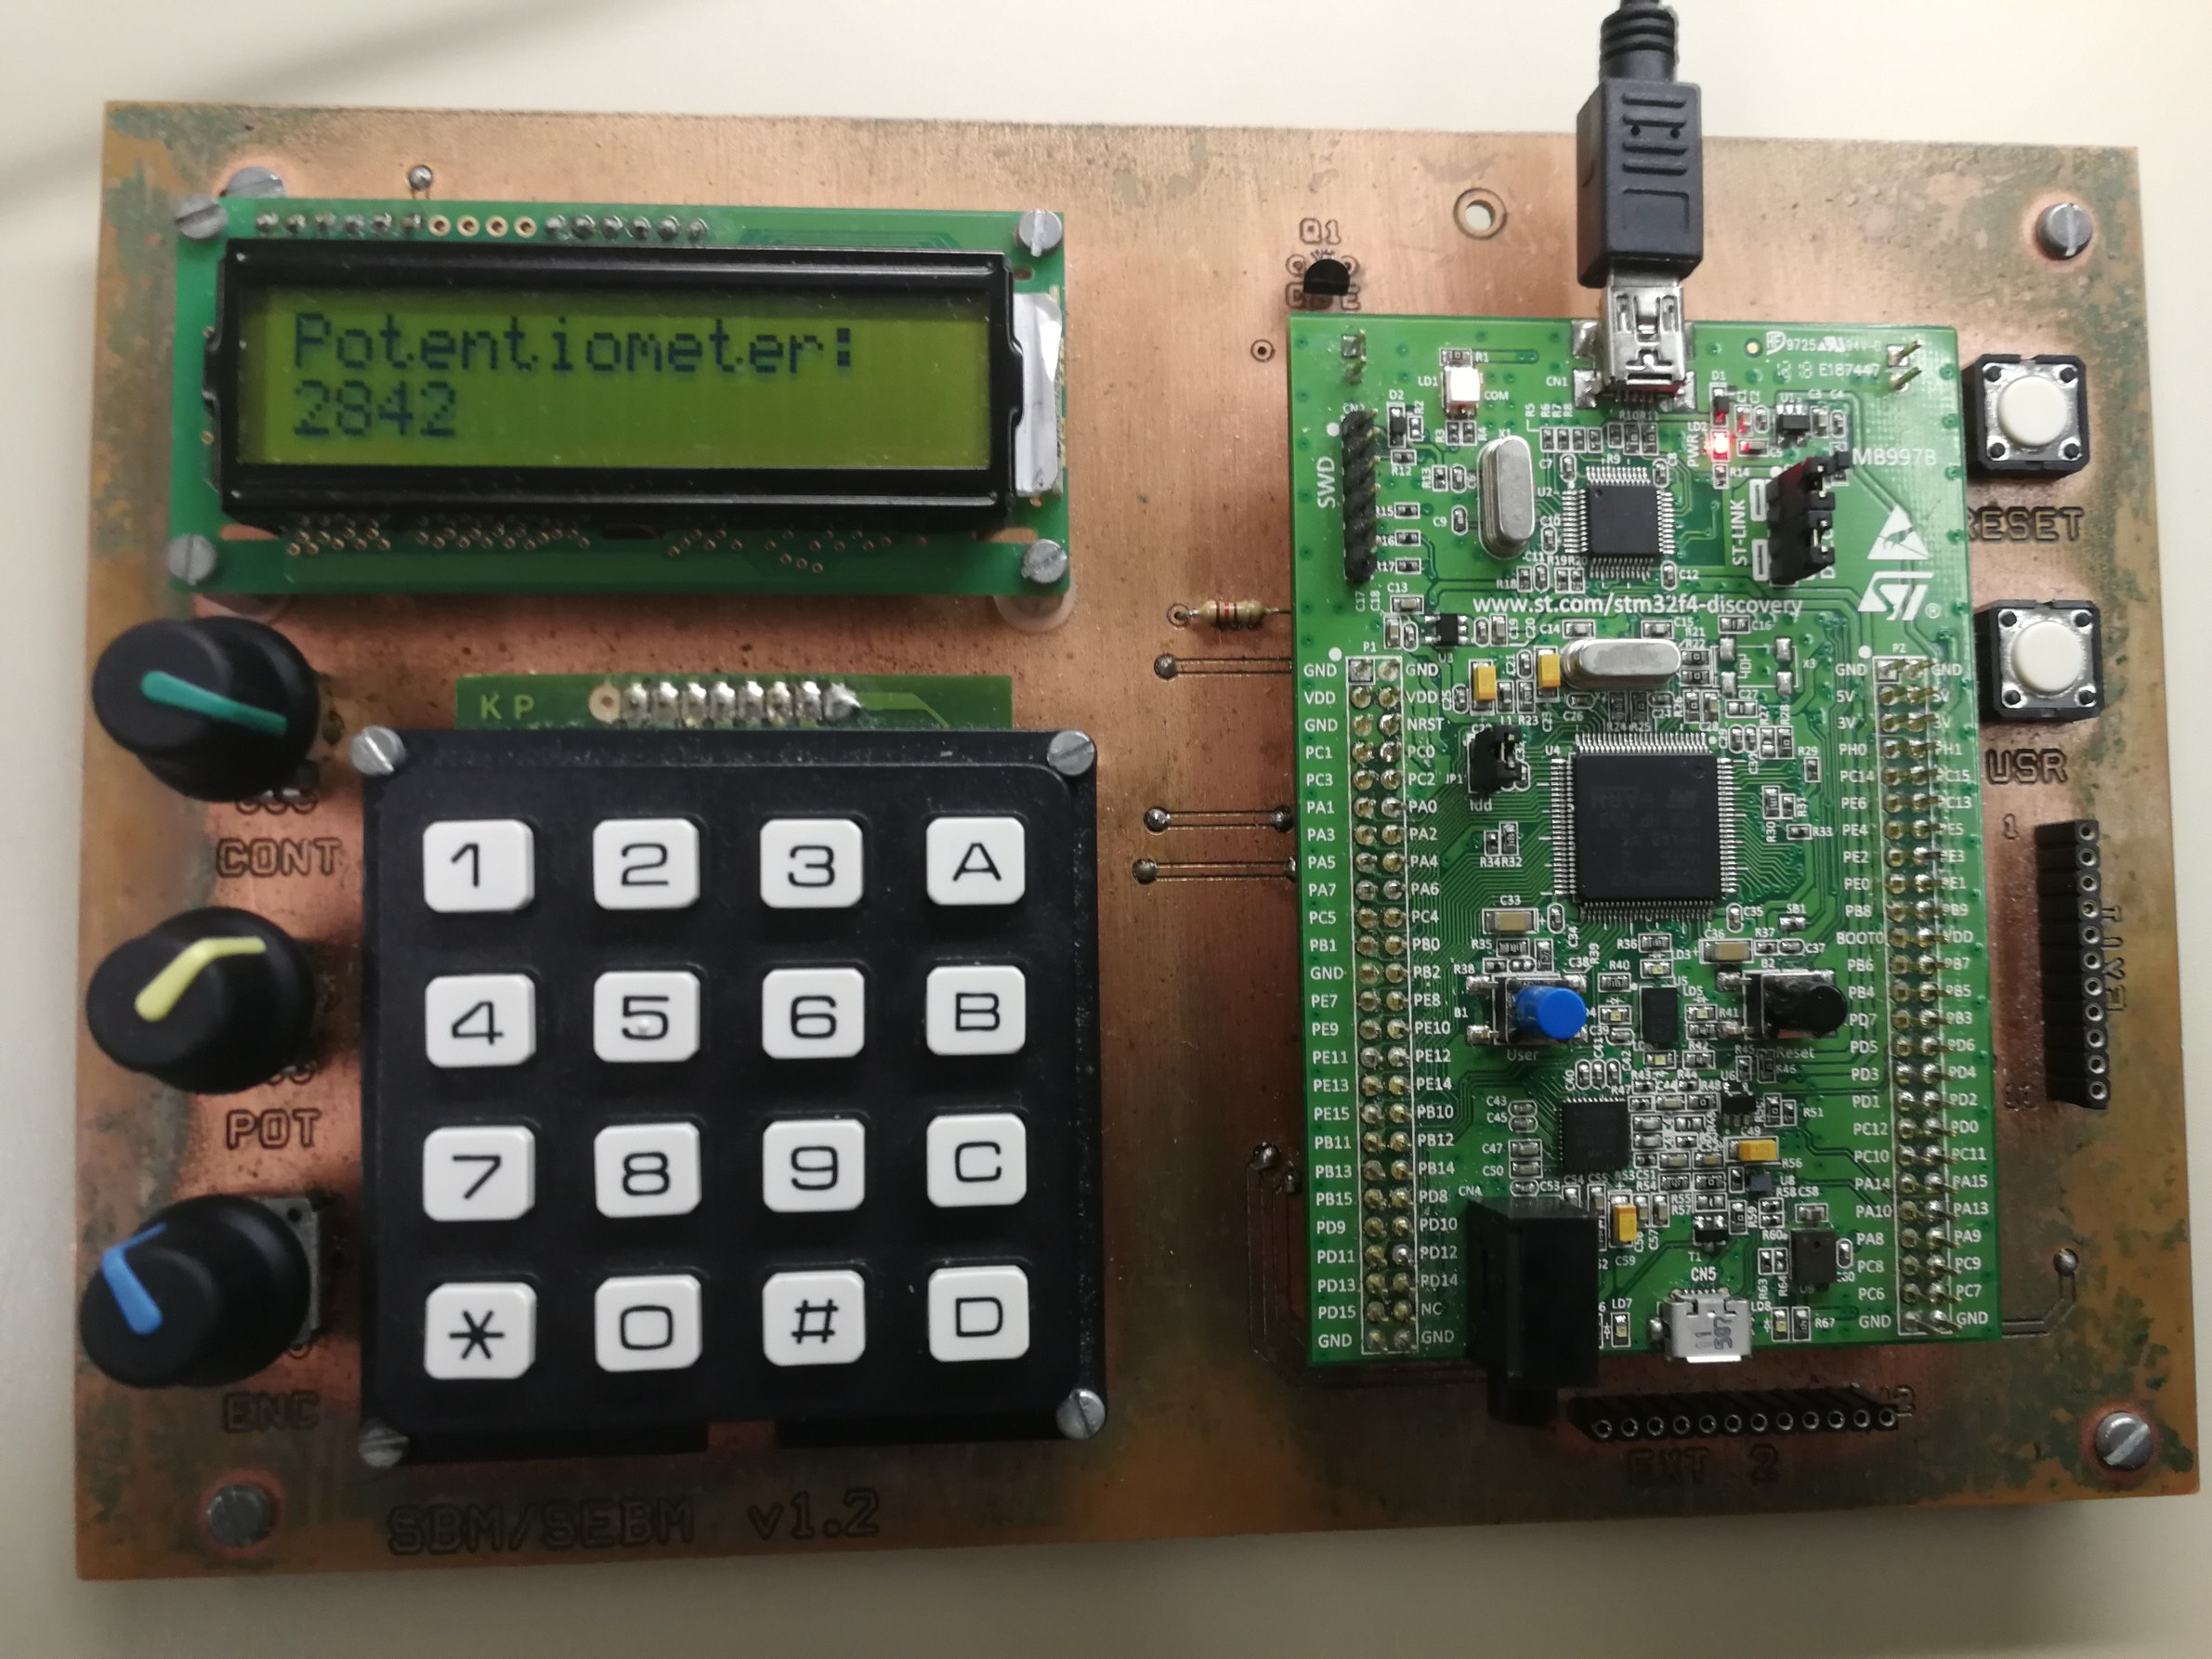
\includegraphics[width=.99\columnwidth]{../photos/board/c2-pot-mid}
  \caption{ \label{fig:c2-board-pot-mid} La placa mostrant el valor del potenciòmetre, a meitat de recorregut. }
\end{figure}

\begin{figure}[p] %FIXME: subfigures?
  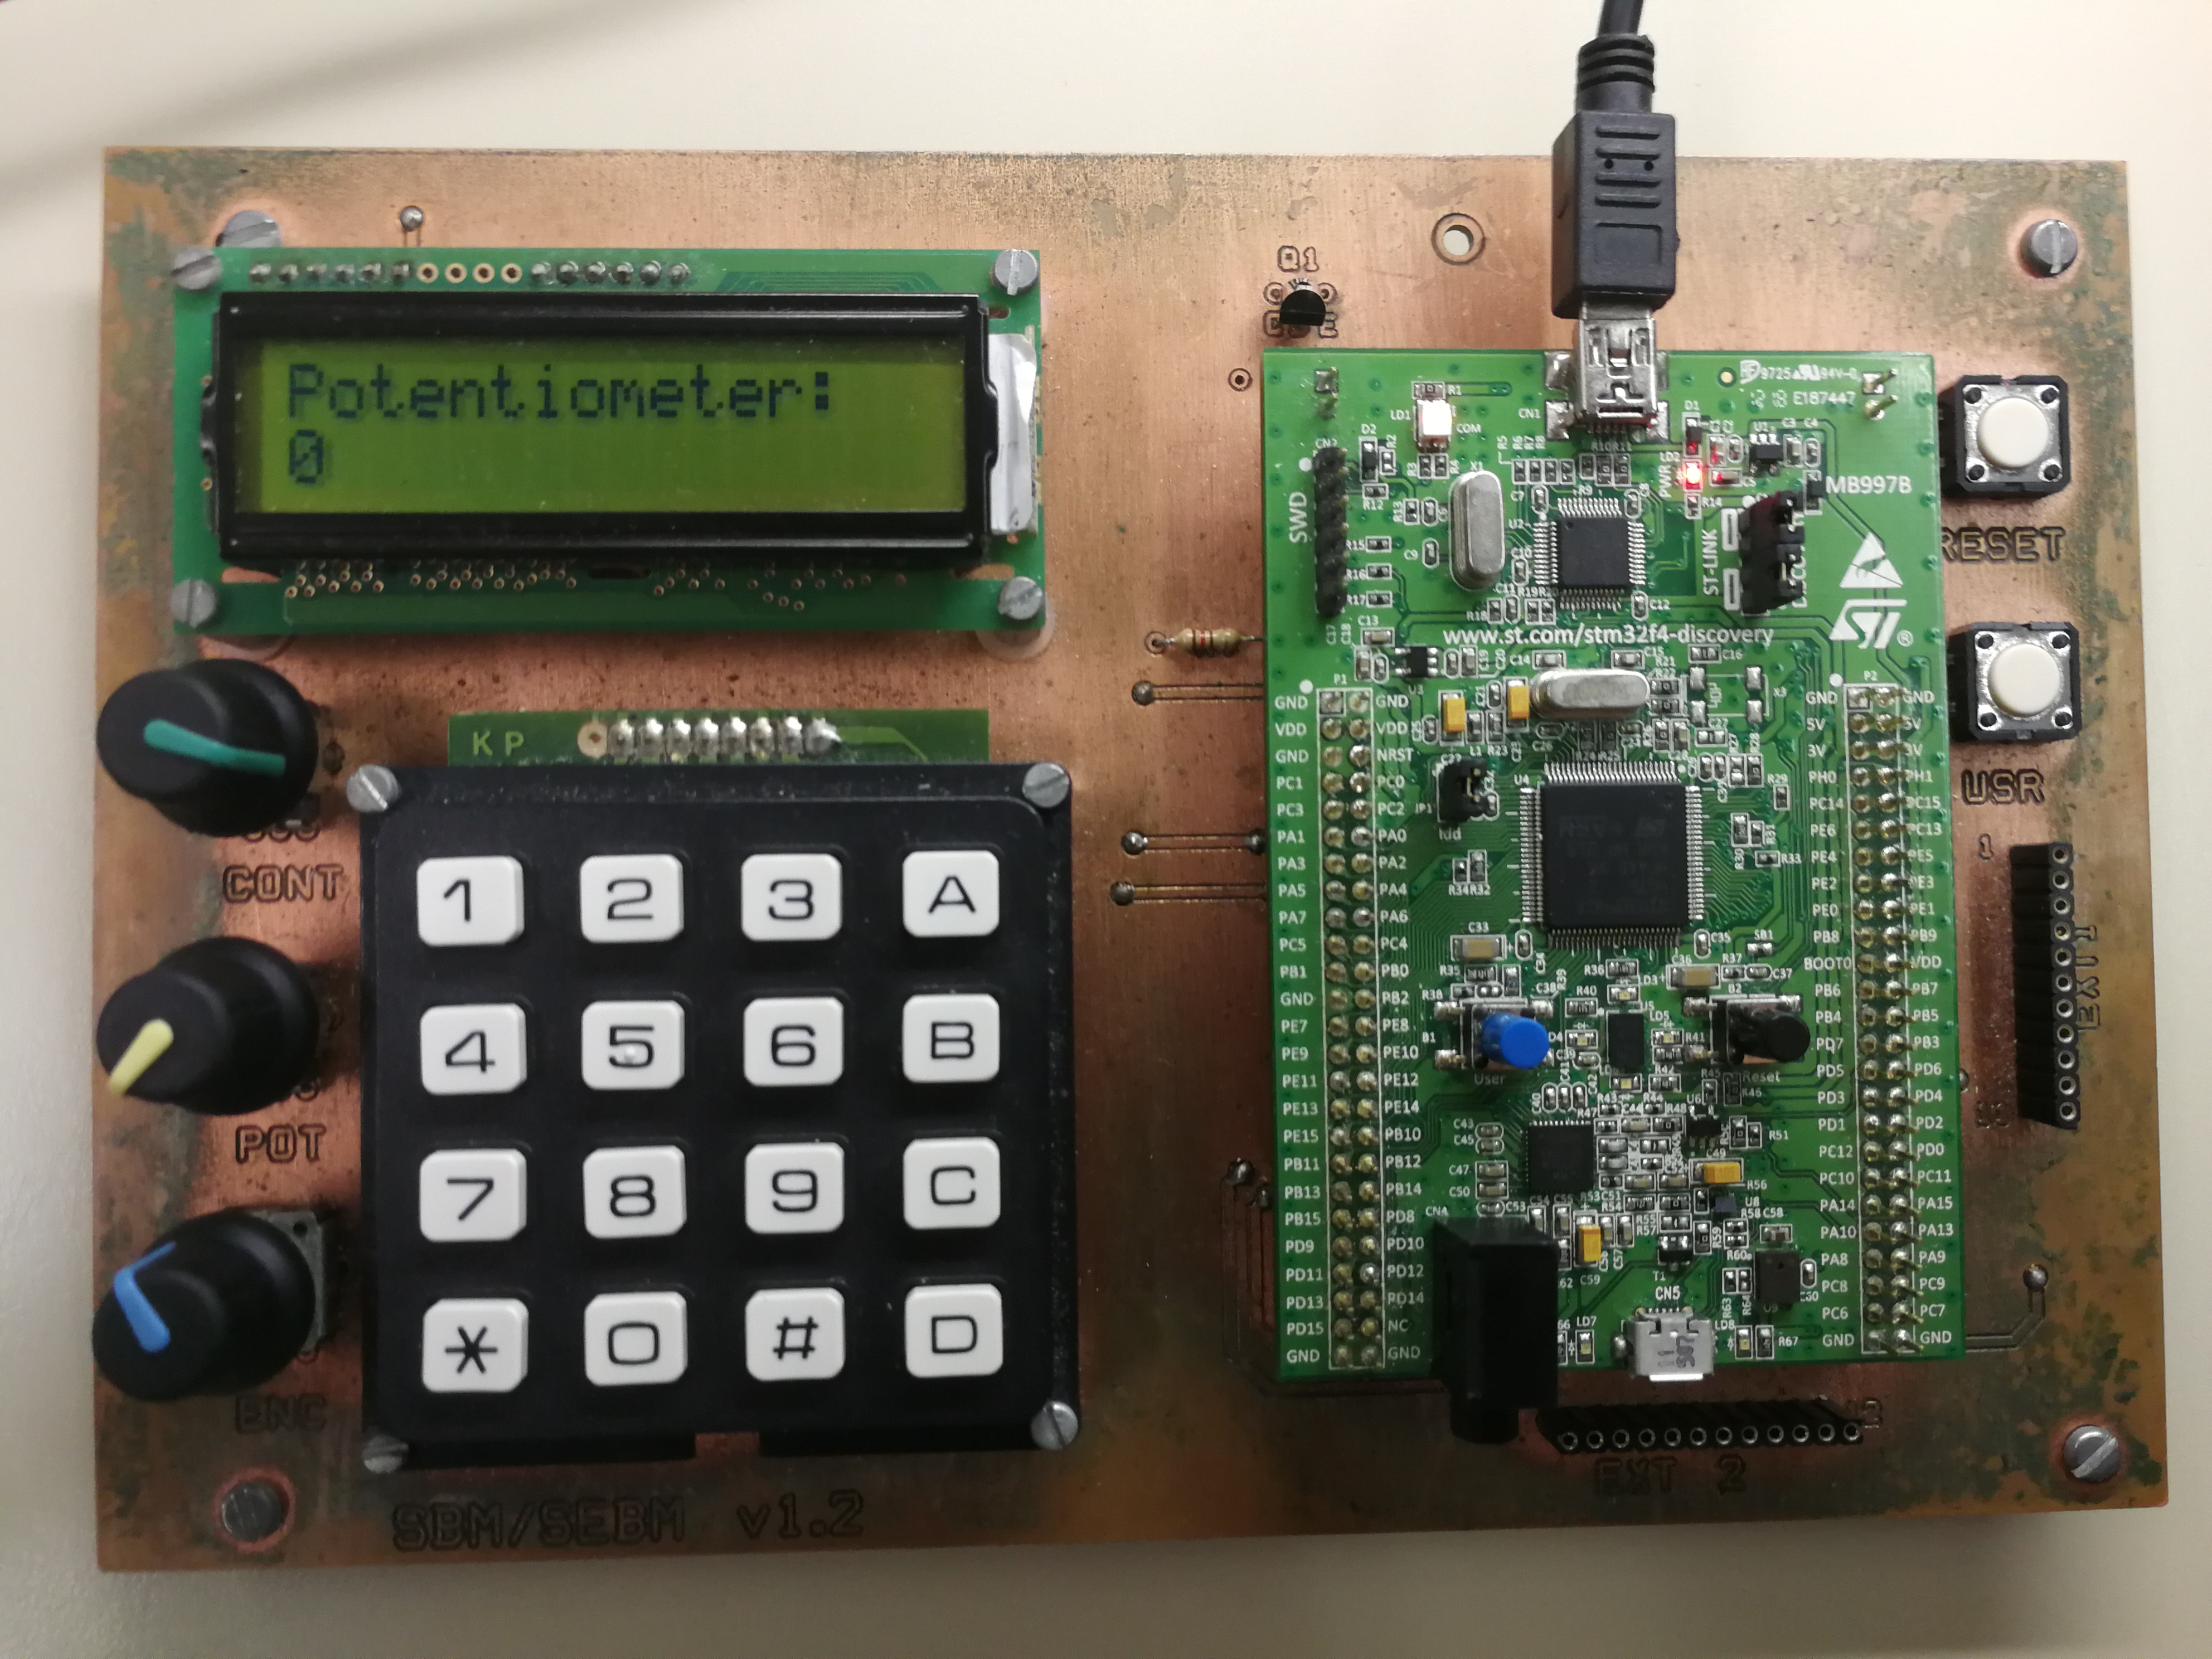
\includegraphics[width=.82\columnwidth]{../photos/board/c2-pot-zero_1}
  \caption{ \label{fig:c2-board-pot-zero} La placa mostrant el valor del potenciòmetre, al mínim. }
\end{figure}
\begin{figure}[p]
  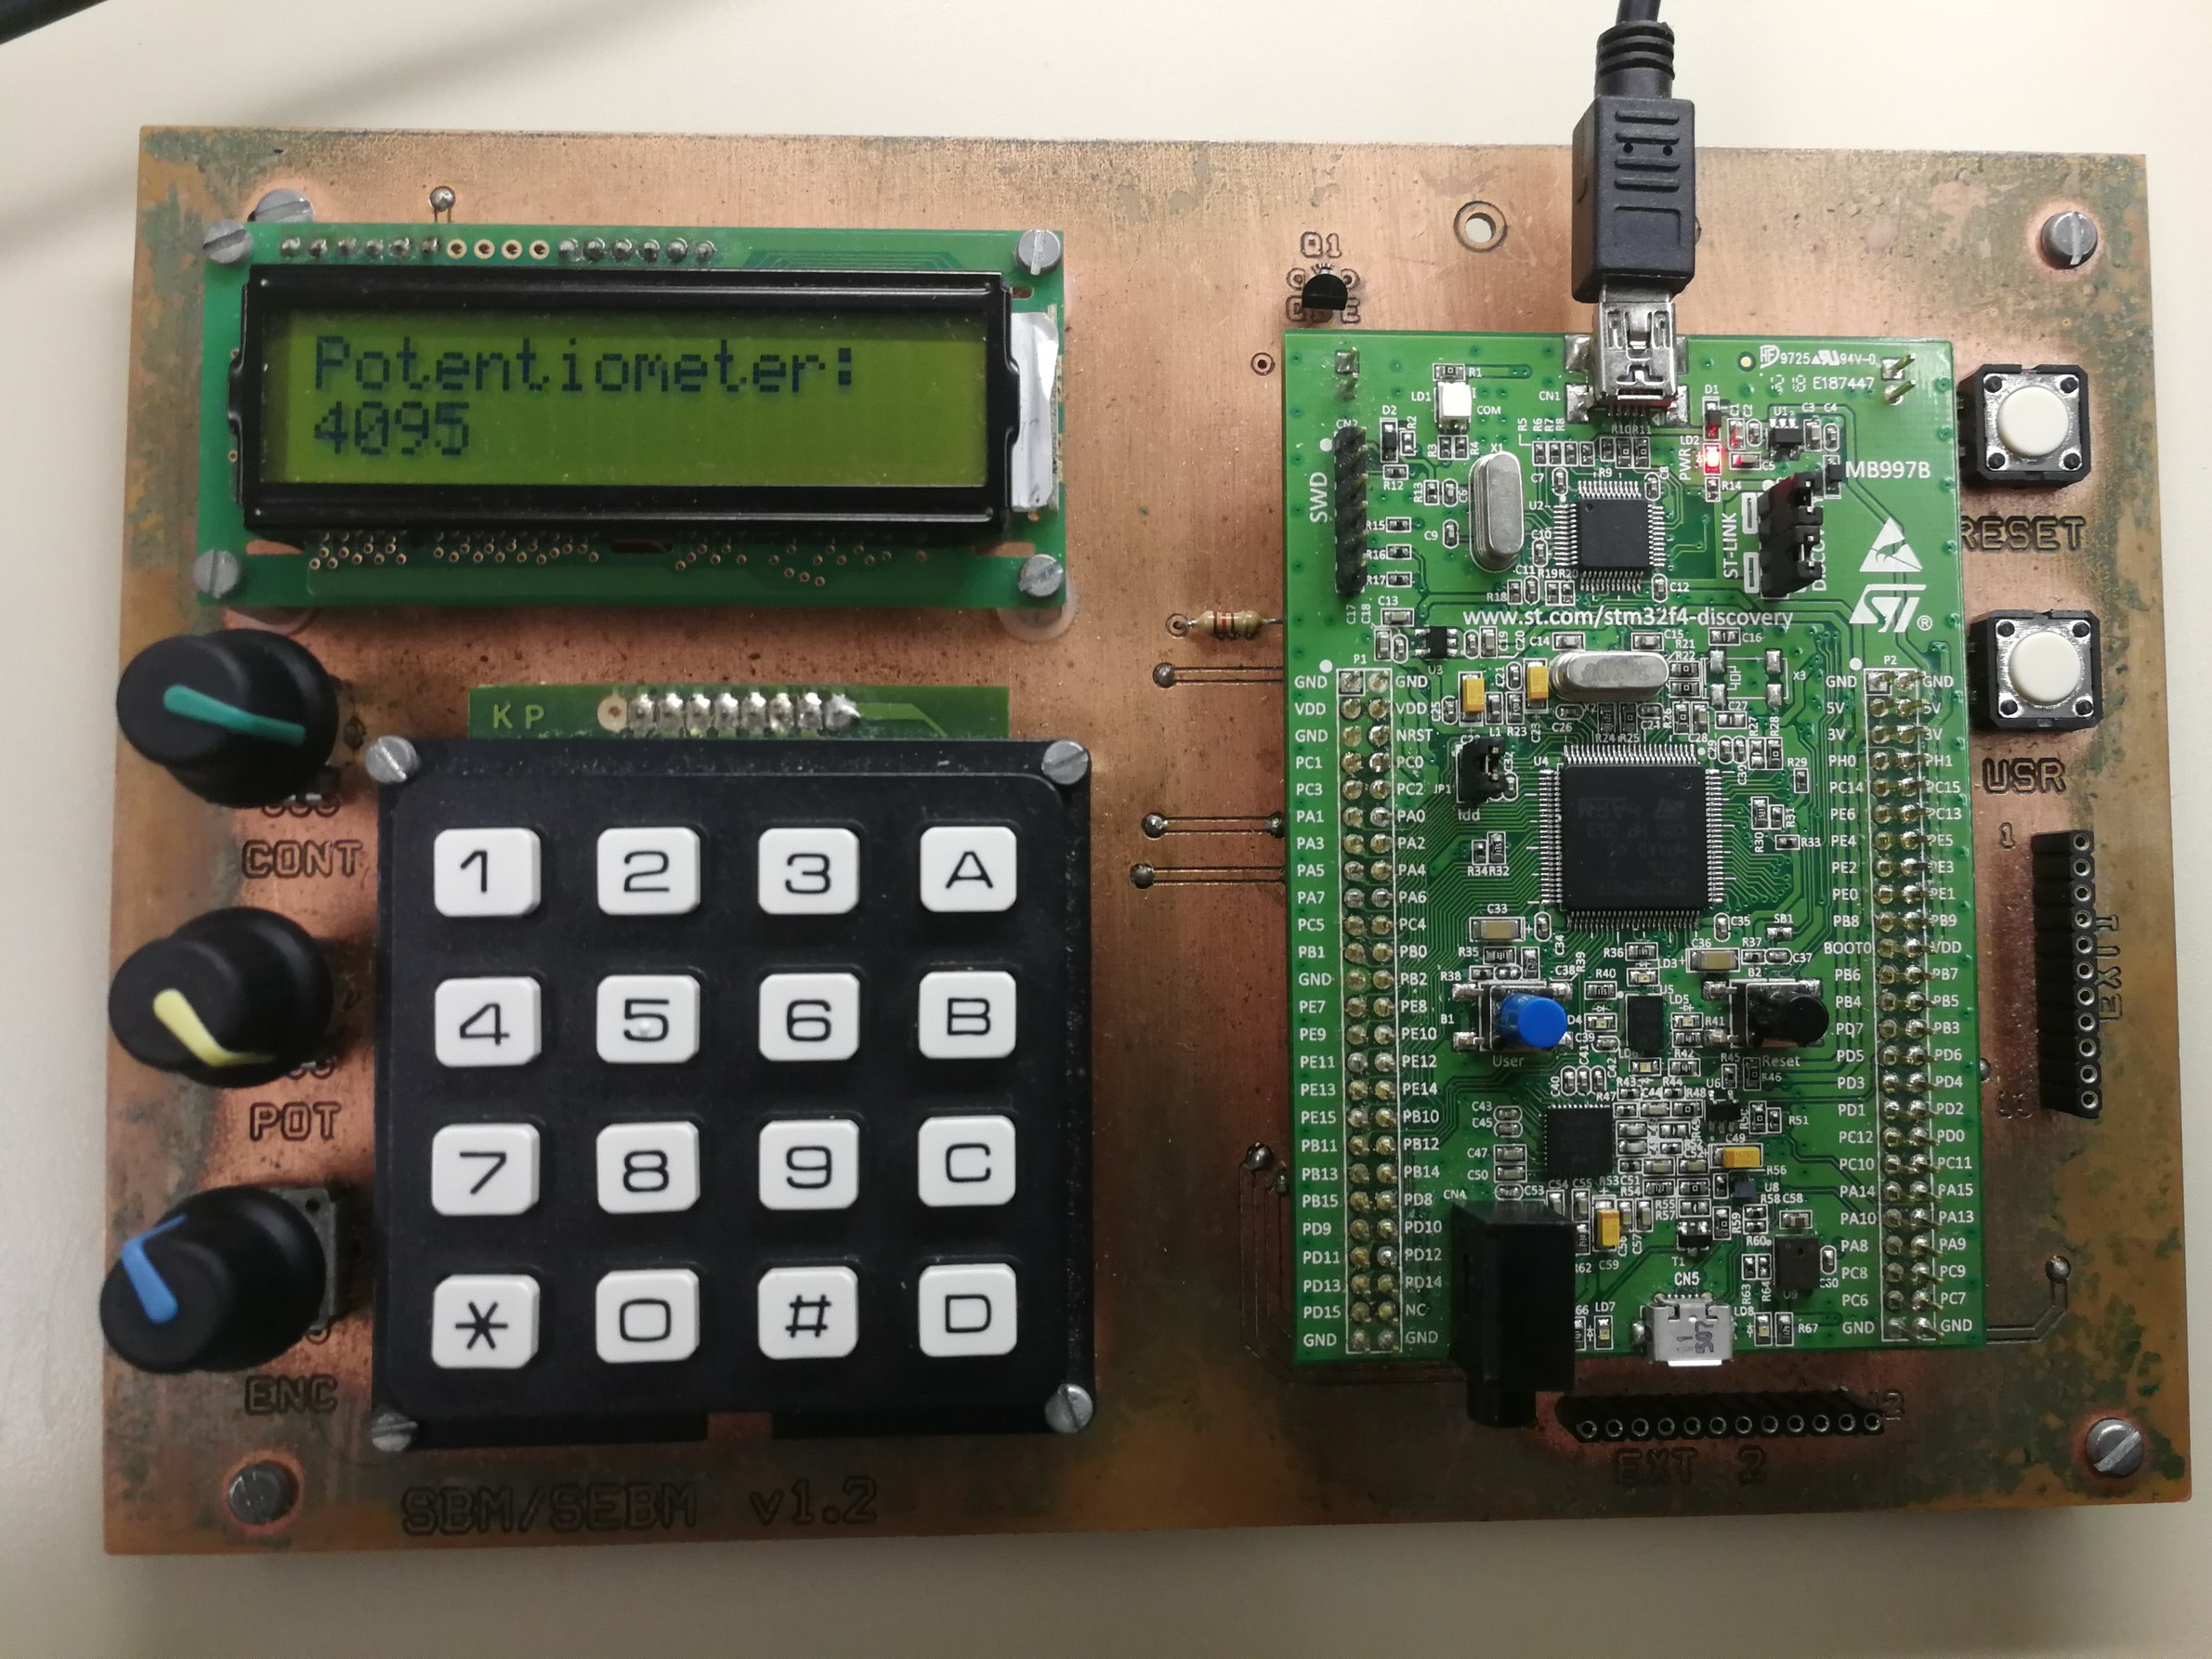
\includegraphics[width=.82\columnwidth]{../photos/board/c2-pot-full}
  \caption{ \label{fig:c2-board-pot-full} La placa mostrant el valor del potenciòmetre, al màxim. }
\end{figure}

Això conforma el \commit{385cc48ae416f2609f8624fec38a5e76584e7f03}.


\subsection{Lectura de la temperatura del microcontrolador}

Ara es llegirà el canal IN16, que és intern i es troba connectat al
sensor de temperatura del microcontrolador. En primer lloc es descriu
la relació del voltatge llegit amb la temperatura del sensor com:

\begin{equation*}
T (\si{\celsius}) = \SI{25}{\celsius} + \frac{V_{sense} - V_{25}}{\mathsf{Avg\_Slope}}
\end{equation*}

On els valors de $V_{25}$ i $\mathsf{Avg\_Slope}$ venen donats a la datasheet
del microcontrolador. Allà també s'hi explica el temps mínim de lectura que
cal tenir.

A continuació cal modificar (estudi previ) la funció \fname{initADC} per fer la inicialització
d'aquest canal i encendre el sensor de temperatura. Finalment, fer una funció
\fname{readT} que realitzi una lectura i retorni la temperatura en dècimes
de grau, fent servir només enters per al càlcul i sense perdre precisió:

%previ
A la funció \fname{initADC} s'han afegit les línies següents abans d'activar ADON:
%
\begin{minted}[mathescape]{c}
    // ...

    // Enable VREFINT and temperature sensor
    ADC->CCR |= ADC_CCR_TSVREFE;
    // Program sample time for IN16 (T) to ensure > $\SI{10}{\micro\second}$
    ADC1->SMPR1 = (ADC1->SMPR1 & (~ADC_SMPR1_SMP16)) | ADC_SMPR1_SMP_SENSOR(ADC_SAMPLE_480);

    // Power up ADC1
    // ...
\end{minted}
\vskip -1em

I la funció \fname{readT} s'ha definit amb ajuda d'algunes constants, així:

\begin{minted}[mathescape]{c}
// Temperature sensor values from datasheet
#define TS_AVG_SLOPE     25 // $\si{\milli\volt}$ increment every $\SI{10}{\celsius}$
#define TS_V25          760 // $\si{\milli\volt}$ at $\SI{25}{\celsius}$

// Read the internal temperature sensor; returned
// value is in tenths of Celsius degrees
int32_t readT(void) {
    // Read the temperature sensor
    int32_t vsense = readChannel(ADC_CHANNEL_SENSOR);

    // Calculate $T = 250 + \frac{\text{vsense} / 4095 \, V_{dd} - V_{25}}{\text{TS\_AVG\_SLOPE} / 100}$
    // Which results in $T = 250 + 100 \frac{\text{vsense} V_{dd} - 4095 \, V_{25}}{4095 \, \text{TS\_AVG\_SLOPE}}$
    return 250 + (100 * (vsense * 3000 - 4095 * TS_V25)) / (4095 * TS_AVG_SLOPE);
}
\end{minted}
\vskip -1em
%/previ

A continuació s'introdueix el codi i s'escriu un programa que llegeix periòdicament
el valor de temperatura i el mostra a la pantalla, formatat adequadament amb una
xifra de precisió:

\begin{minted}{c}
void temperaturePoll(void) {
    uint8_t degree [] = {
        0b00000110,
        0b00001001,
        0b00001001,
        0b00001001,
        0b00000110,
        0b00000000,
        0b00000000,
        0b00000000,
    };
    LCD_CustomChar(2, degree);
    LCD_ClearDisplay();
    LCD_SendString("Temperature:");
    LCD_Config(TRUE, FALSE, FALSE);

    while (1) {
        // Read temperature and convert to string
        int32_t t = readT();
        char tStr [8];
        itoa_fix(t, tStr, 10, 1);

        // Write at display
        LCD_GotoXY(0, 1);
        LCD_SendString(tStr);
        LCD_SendString(" \x02""C  ");

        // Wait before next refresh
        SLEEP_MS(200);
    }
}
\end{minted}
\vskip -1em

\voluntari
Per fer el formateig d'un nombre de coma fixa podriem
fer-lo amb \fname{itoa} i tallar els caràcters manualment, però és
complex i hi ha diversos casos a gestionar.

Per tant s'ha decidit fer una còpia d'aquesta funció que pugui treballar
amb nombres en coma fixa, que hem anomenat \fname{itoa_fix}:

\begin{minted}{c}
// Fixed point number to string conversion in the given radix
//      num:   Number to convert
//      str:   Pointer to the string where the result should be located
//               the user should reserve the needed space fo the string.
//      radix: Radix to use. Typically it will be:
//                  2  Binary
//                  10 Decimal
//                  16 Hexadecimal
//      fixed: Amount of digits to show after the dot
char *itoa_fix(int32_t num, char *str, int32_t radix, int32_t fixed);
\end{minted}
\vskip -1em

I s'implementa com segueix:

\begin{minted}{c}
char *itoa_fix(int32_t num, char *str, int32_t radix, int32_t fixed) {
    int32_t sign = 0;   // To remember the sign if negative
    int32_t pos = 0;    // String position
    int32_t i;          // Generic use variable

    //Save sign
    if (num < 0) {
        sign = 1;
        num = -num;
    }

    //Construct a backward string of the number.
    do {
        i = num % radix;
        if (i < 10)
            str[pos] = i + '0';
        else
            str[pos] = i - 10 + 'A';
        pos++;
        num /= radix;

        if (fixed > 0 && pos == fixed) {
            str[pos] = '.';
            pos++;
        }
    }    while (num > 0 || pos <= fixed);

    //Now add the sign
    if (sign)
        str[pos] = '-';
    else
        pos--;

    // Add the final null
    str[pos + 1] = 0;

    // Pos is now the position of the final digit (before null)

    // Now reverse the string
    i = 0;
    do {
        sign = str[i];
        str[i++] = str[pos];
        str[pos--] = sign;
    } while (i < pos);

    return str;
}
\end{minted}
\vskip -1em

El programa es carrega a la placa i es verifica el correcte funcionament.
El resultat es pot veure a la figura~\ref{fig:c2-board-temp}. Cal notar que la temperatura
fluctua unes quantes dècimes en cada lectura.

\begin{figure}
  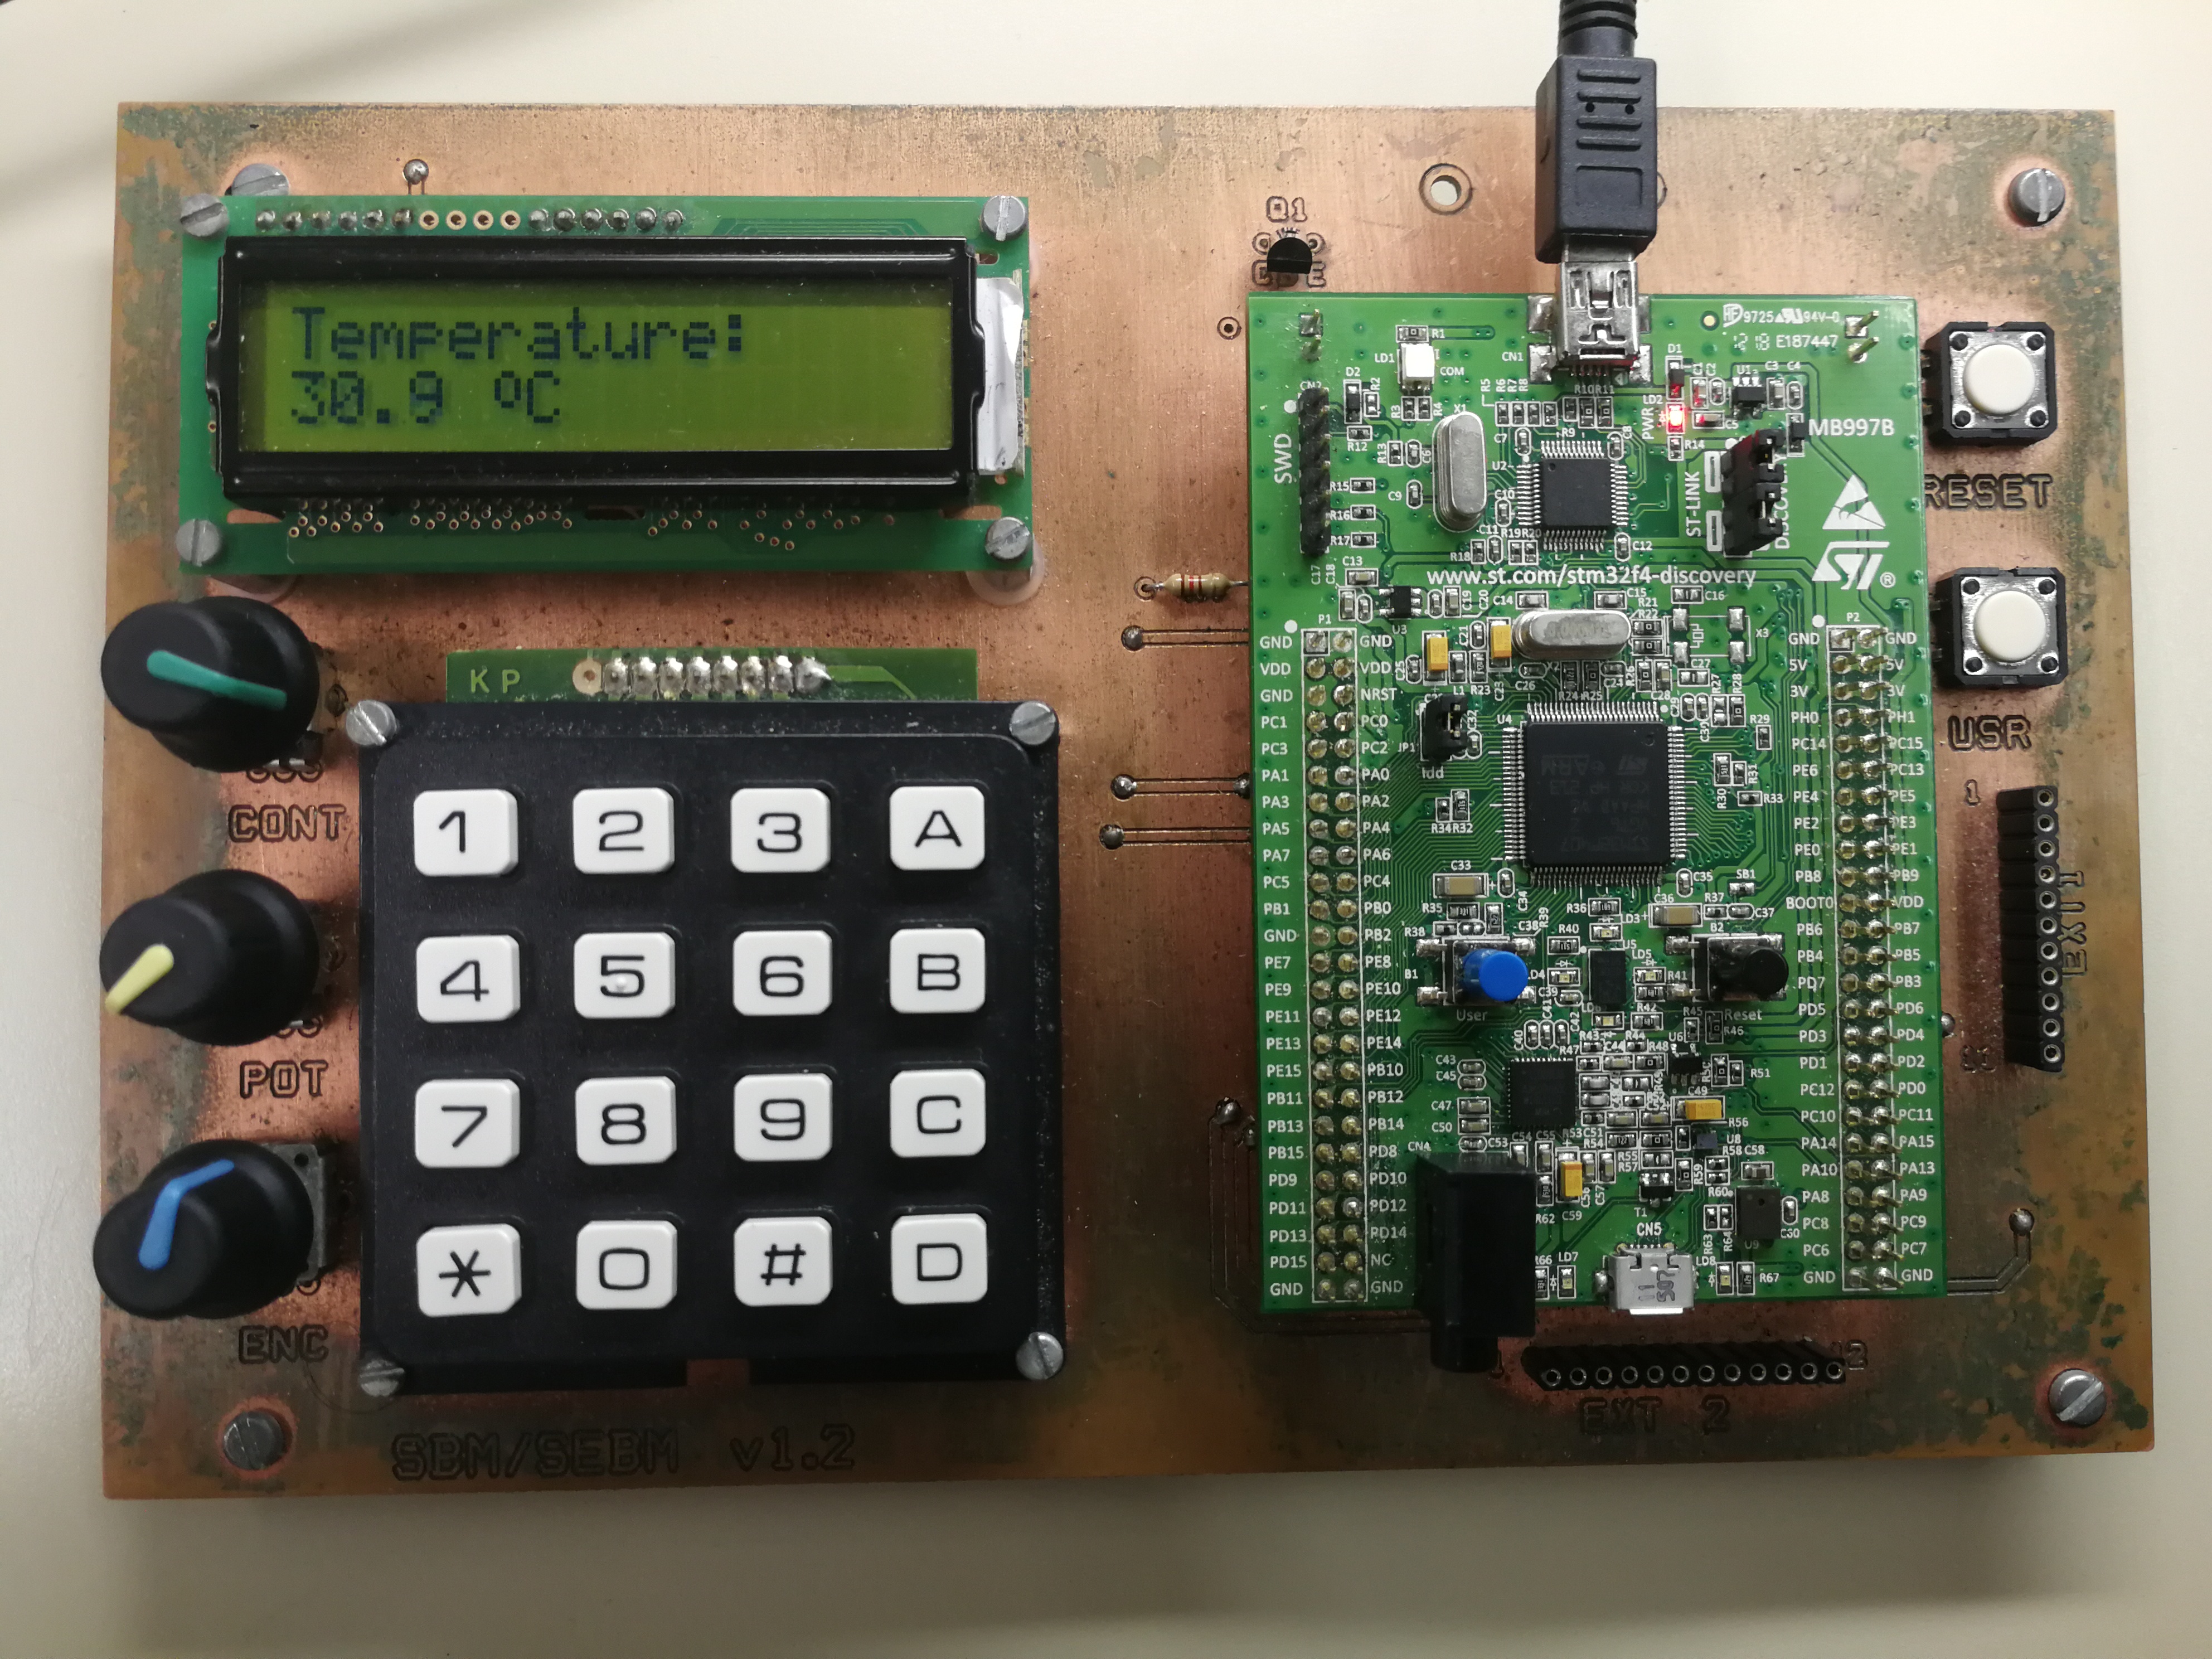
\includegraphics[width=.99\columnwidth]{../photos/board/c2-temp-2}
  \caption{ \label{fig:c2-board-temp} La placa mostrant la lectura del sensor de temperatura. }
\end{figure}

Això conforma el \commit{bfbcae30458e316cb9507ae429780dc70668473a}.


\subsection{Calibrat de l'ADC}

S'exposa ara la possibilitat de llegir la referència de tensió, que està connectada
a IN17 i té un voltatge conegut de forma molt més precisa. D'aquí podem deduir $V_{DD}$,
i per tant sabrem quina és a referència exacta quan fem mesures en altres canals.

D'entrada, hem de configurar el canal IN17 amb el temps de lectura apropiat segons
el datasheet:

\begin{minted}[mathescape]{c}
    // ...

    // Enable VREFINT and temperature sensor
    ADC->CCR |= ADC_CCR_TSVREFE;
    // Program sample time for IN16 (T) and IN17 (VREFINT) to ensure > $\SI{10}{\micro\second}$
    ADC1->SMPR1 = (ADC1->SMPR1 & (~ADC_SMPR1_SMP16)) | ADC_SMPR1_SMP_SENSOR(ADC_SAMPLE_480);
    ADC1->SMPR1 = (ADC1->SMPR1 & (~ADC_SMPR1_SMP17)) | ADC_SMPR1_SMP_VREF(ADC_SAMPLE_480);

    // Power up ADC1
    // ...
\end{minted}
\vskip -1em

No cal encendre la referència de tensió perquè el bit per habilitar-la és el mateix
que per al sensor de temperatura i, per tant, ja es va habilitar en la secció anterior.

Es demana llavors, com a estudi previ, elaborar una funció \fname{readVdd} que realitzi una lectura
de la tensió de referència i a partir d'aquí, retorni $V_{DD}$ en \si{mV}. Igual que per a
\fname{readT}, la funció no ha de fer servir coma flotant en els càlculs i s'ha d'anar amb
cura de no perdre precisió. S'implementa com segeix:

%previ
\begin{minted}[mathescape]{c}
// Voltage reference values from datasheet [$\si{mV}$]
#define VREFINT_MIN 1180
#define VREFINT_TYP 1210
#define VREFINT_MAX 1240

// Using the ADC voltage reference, return Vdd voltage
// in millivolts
int32_t readVdd(void) {
    // Read the voltage reference
    int32_t vrefint = readChannel(ADC_CHANNEL_VREFINT);

    // Calculate Vdd knowing $\text{vrefint} = 4095 \, \frac{V_{REFINT}}{V_{DD}} \Leftrightarrow V_{DD} = 4095 \, \frac{V_{REFINT}}{\text{vrefint}}$
    return (4095 * VREFINT_TYP) / vrefint;
}
\end{minted}
%/previ

S'insereix el codi de la funció a \filename{analog.c} i s'escriu un petit programa
que llegeix periòdicament el valor de $V_{DD}$ i el mostra a la pantalla, degudament
formatejat:

\begin{minted}{c}
void vddPoll(void) {
    LCD_ClearDisplay();
    LCD_SendString("Vdd =");
    LCD_Config(TRUE, FALSE, FALSE);

    while (1) {
        // Read temperature and convert to string
        int32_t vdd = readVdd();
        char vddStr [8];
        itoa_fix(vdd, vddStr, 10, 3);

        // Write at display
        LCD_GotoXY(6, 0);
        LCD_SendString(vddStr);
        LCD_SendString(" V");

        // Wait before next refresh
        SLEEP_MS(200);
    }
}
\end{minted}
\vskip -1em

Es puja el codi a la placa i es verifica el seu correcte funcionament.
El resultat es pot veure a la figura~\ref{fig:c2-board-vdd}.
Això conforma el \commit{c4db75f712f4ff0f91c3f4a5bca2b074dba55cc7}.

\begin{figure}
  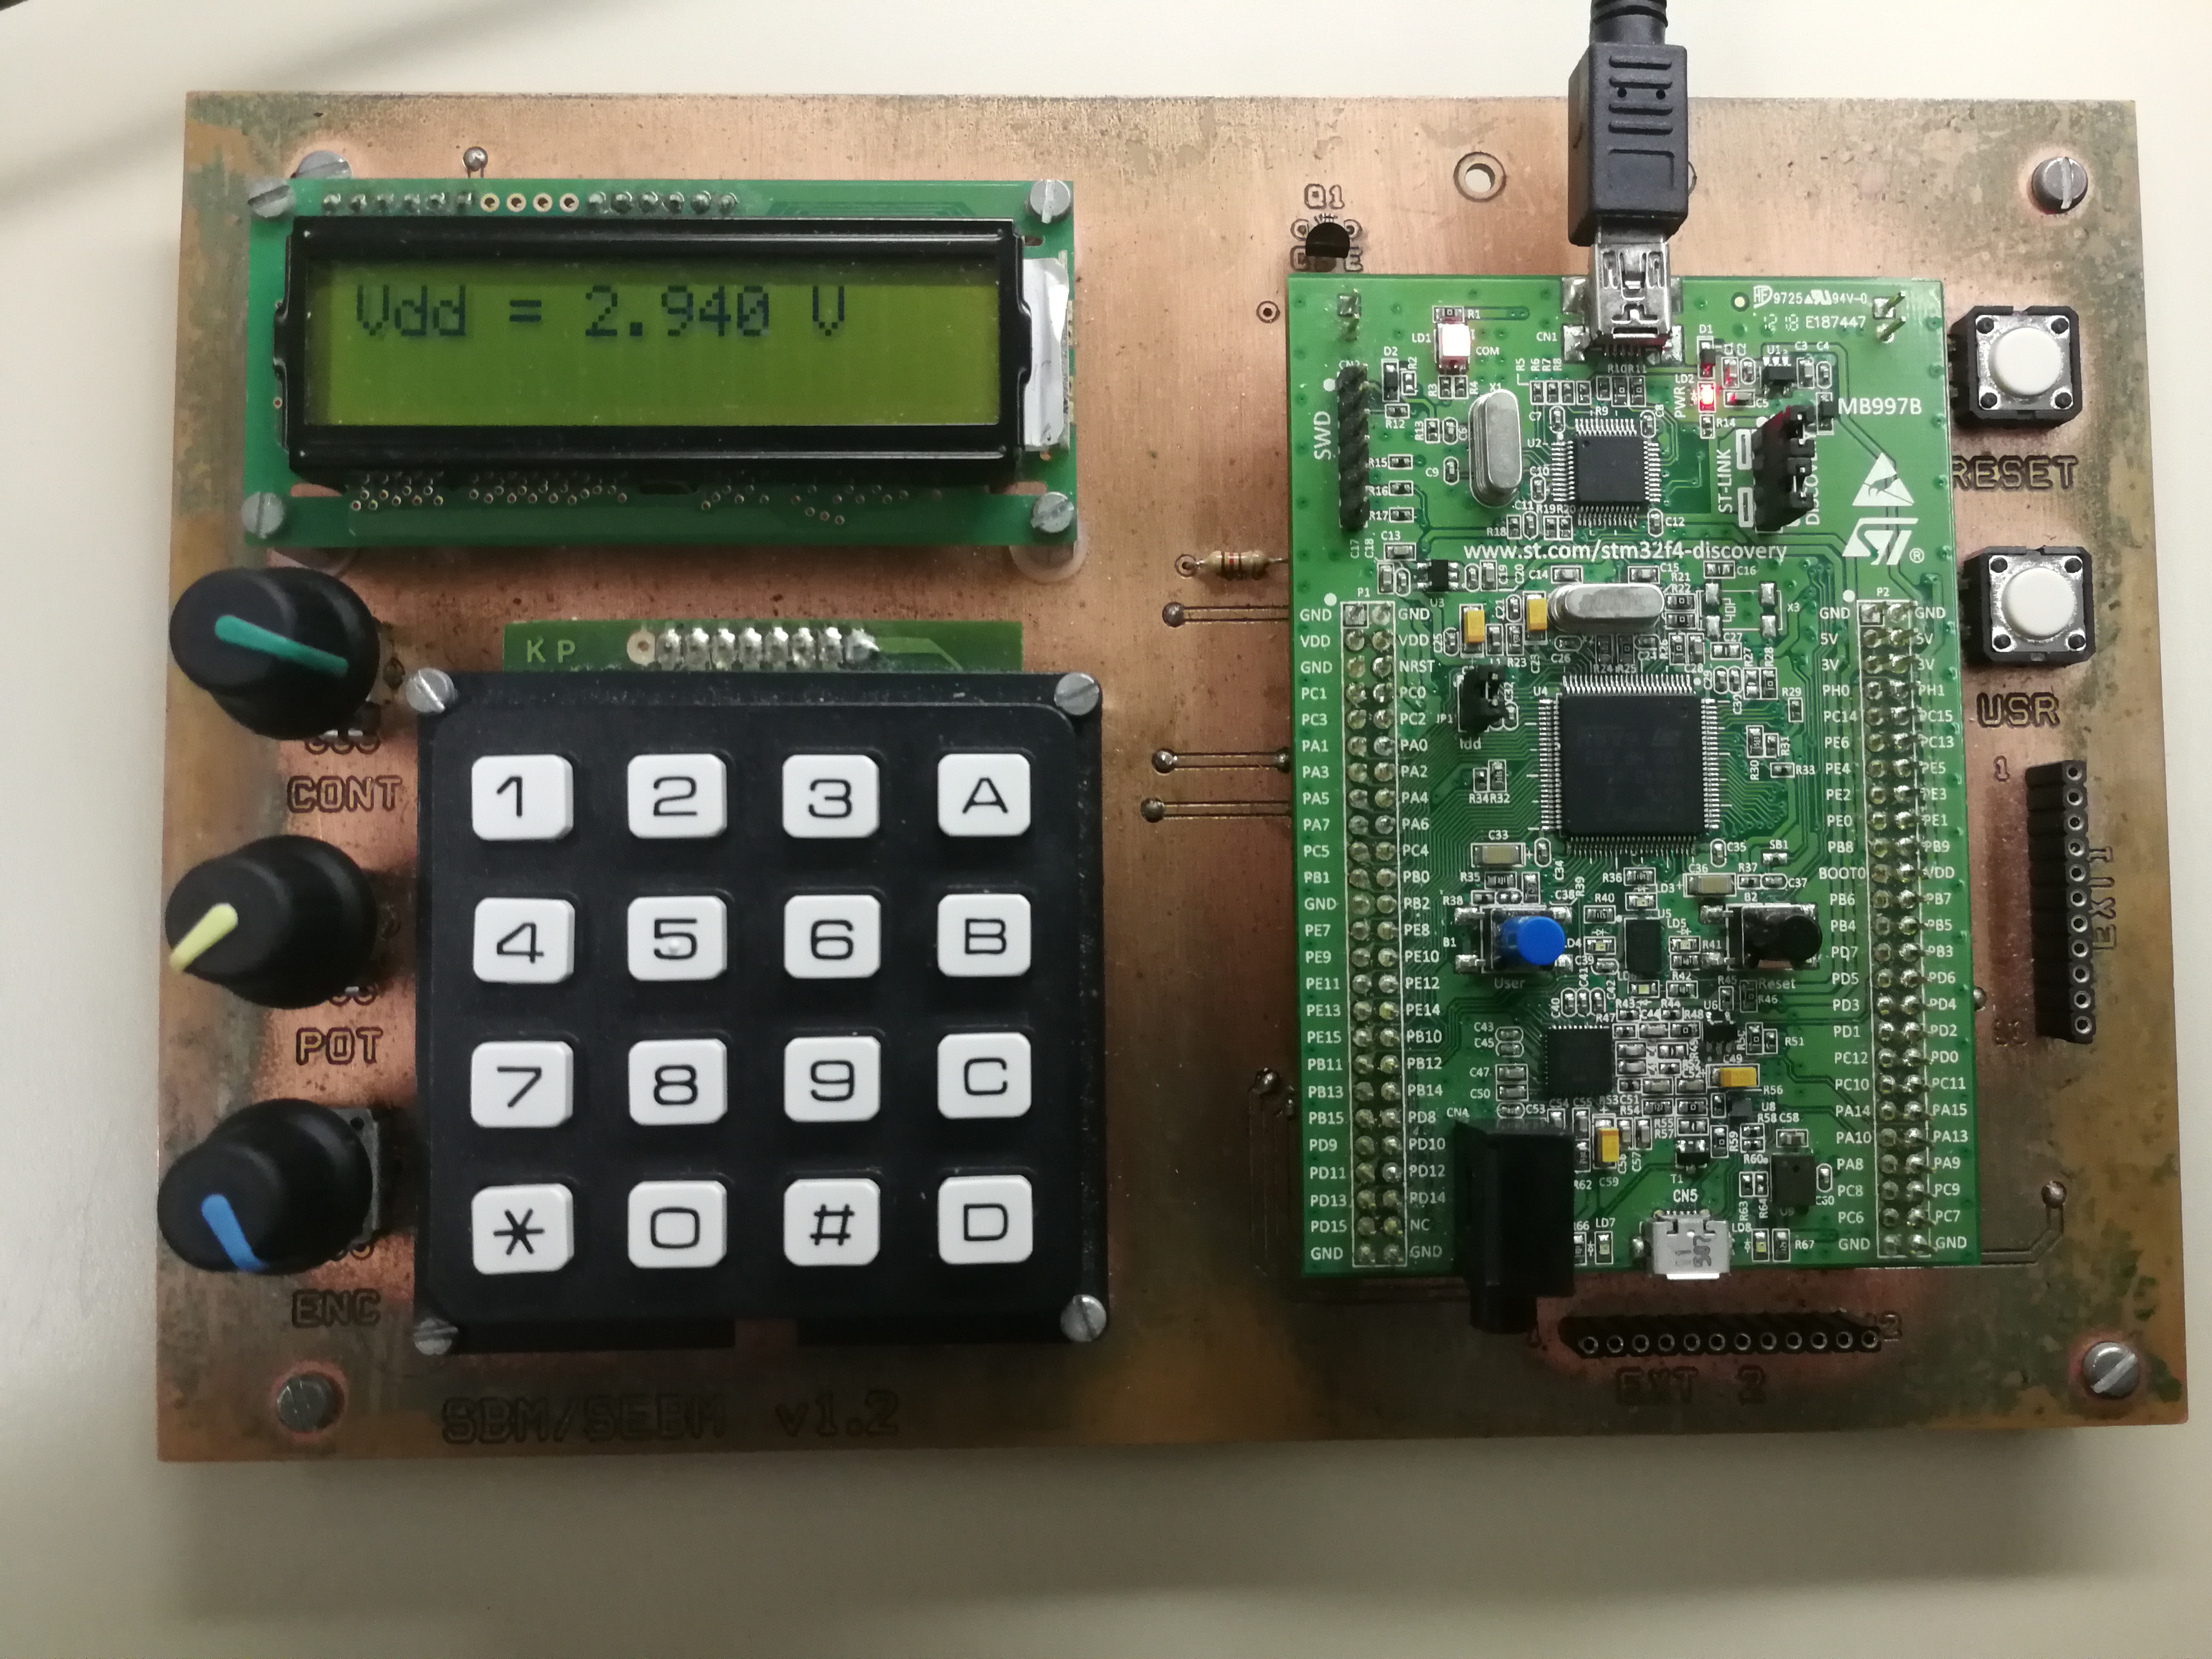
\includegraphics[width=.99\columnwidth]{../photos/board/c2-vdd_1}
  \caption{ \label{fig:c2-board-vdd} La placa mostrant la lectura de la tensió d'alimentació. }
\end{figure}

\opcional
Ara farem servir les lectures de $V_{DD}$ per calibrar les lectures de
temperatura del sensor. Per fer-ho, modificarem \fname{readT} perquè cridi
\fname{readVdd} i faci servir aquest resultat en comptes de la constant
$3000$ que s'emprava prèviament. La funció \fname{readT} queda així:

\begin{minted}[mathescape]{c}
// Temperature sensor values from datasheet
#define TS_AVG_SLOPE     25 // $\si{\milli\volt}$ increment every $\SI{10}{\celsius}$
#define TS_V25          760 // $\si{\milli\volt}$ at $\SI{25}{\celsius}$

// Read the internal temperature sensor; returned
// value is in tenths of Celsius degrees
int32_t readT(void) {
    // Read the temperature sensor and $V_{DD}$
    int32_t vsense = readChannel(ADC_CHANNEL_SENSOR);
    int32_t vdd = readVdd();

    // Calculate $T = 250 + \frac{\text{vsense} / 4095 \, V_{dd} - V_{25}}{\text{TS\_AVG\_SLOPE} / 100}$
    // Which results in $T = 250 + 100 \frac{\text{vsense} V_{dd} - 4095 \, V_{25}}{4095 \, \text{TS\_AVG\_SLOPE}}$
    return 250 + (100 * (vsense * vdd - 4095 * TS_V25)) / (4095 * TS_AVG_SLOPE);
}
\end{minted}
\vskip -1em


\section{Conclusió}

Pràctica molt entretinguda! Excepte per una mica de confusió
fent les operacions de calibració de l'ADC i el sensor de temperatura,
la pràctica s'ha desenvolupat sense problemes.

\section{Ajustaments posteriors}

Cap canvi a destacar.
